\appendix
\part*{Annexes}
\addcontentsline{toc}{part}{Annexes}
\pagestyle{myheadings}
\markboth{Annexes}{Annexes}

\section{Disponibilité des données du mémoire}\label{code}

Illustrations, code et données du mémoire disponibles sur Github à cette adresse : \url{https://github.com/giangpen/B.S.E.I.}. 

Version \LaTeX disponible sur Github, à cette adresse \url{}.

\newpage
\section{LDA topics 12 Sujets}

Topic 0: cachet,caractère,forme,sceau,grand,che,ang,ancien,han,chinois

Topic 1: mer,sud,pays,che,tchen,ang,nord,nom,nan,tan

Topic 2: société,saigon,comité,membre,séance,président,général,etude,secrétaire,bulletin

Topic 3: jarre,vietnam,saigon,perle,van,lao,objet,poterie,forme,tesson

Topic 4: village,nam,viet,system,central,vietnamese,area,social,vith,northern

Topic 5: cau,ang,roi,faire,samtec,troupe,pays,grand,homme,royal

Topic 6: faire,grand,bien,jour,homme,roi,pays,chinois,annamite,lettre

Topic 7: thi,nguy,cho,nam,phong,chi,femme,trong,vietnamien,bien

Topic 8: nguy,grand,année,empereur,mandarin,lê,nam,chinois,tri,faire

Topic 9: eau,petit,grand,art,forme,village,bien,terre,maison,pierre

Topic 10: chinois,paddy,histoire,chine,van,auteur,étude,réf,vietnamien,cochinchine

Topic 11: compte,nam,pari,sud,bien,vietnamien,grand,nom,face,licent


\newpage 
\section{LDA topics 24 Sujets}

Topic 2: chinois,jour,grand,chine,nom,caractère,bien,pays,cachet,date

Topic 10: poste,paillote,xay,délégation,village,phu,xine,milicien,bou,méra

Topic 16: pot,chaux,cuy,chique,annamite,chine,poisson,vai,espèce,anse

Topic 3: association,pinus,pin,classe,social,dalat,chef,structure,réclusion,individu

Topic 13: nam,carte,saigon,vietnamien,nom,société,viet,sud,duong,van

Topic 14: société,pari,tonkin,saigon,géographie,cochinchine,chine,carte,indo,français

Topic 18: jarre,forme,petit,long,objet,poterie,partie,région,terre,perle

Topic 21: arrêté,nhlong,nhoà,sadec,délégation,canton,inspection,càmau,contrainte,luin

Topic 0: rue,face,mélanésien,bien,indice,gauche,facette,bord,crête,européen

Topic 9: fromage,chao,soia,géologique,haricot,azote,mine,sauce,graine,fermenter

Topic 5: saigon,compte,directeur,service,commettre,administrateur,colonial,cochinchine,france,van

Topic 12: chinois,siècle,étude,chine,histoire,grand,art,ancien,pari,sud

Topic 6: monument,art,angkor,siècle,temple,tête,tour,pierre,statue,petit

Topic 19: vith,vietnamese,also,voyel,rhode,letter,vjetnamese,language,vord,system

Topic 11: société,membre,comité,séance,président,saigon,général,faire,bulletin,travail

Topic 23: nguy,nam,thi,grand,lê,vietnamien,chinois,tri,année,texte

Topic 4: paddy,vietnam,kuê,van,lao,saigon,demande,carte,bull,cambodge

Topic 7: faire,grand,bien,siam,fort,eau,roi,pays,français,lettre

Topic 8: tibétain,burnouf,langue,lévi,indianisme,sanskrit,tokharien,sogdien,indien,recherche


Topic 1: annamite,lettre,amiral,faire,saigon,hanoi,commandant,garnier,tonkin,français


\newpage

\newpage
\section{10 topic Top2Vec single word learning}

Keyword topic 0 : ['lecteur' 'pensée' 'savant' 'étudier' 'historien' 'civilisation'
 'scientifique' 'intellectuel' 'auteur' 'ouvrage' 'contemporain' 'notion'
 'critique' 'histoire' 'science' 'conception' 'connaissance' 'historique'
 'progrès' 'littéraire']

Keyword topic 1 : ['surface' 'liquide' 'sec' 'couche' 'mètre' 'diamètre' 'épaisseur' 'sol'
 'profondeur' 'tige' 'quantité' 'matière' 'préparation' 'procédé' 'varier'
 'espèce' 'végétal' 'rare' 'fabrication' 'recouvrir']

Keyword topic 2 : ['comité' 'membre' 'bulletin' 'secrétaire' 'président' 'séance' 'réunion'
 'assemblée' 'publication' 'commission' 'société' 'muser' 'indochinois'
 'budget' 'activité' 'bibliothèque' 'malleret' 'proposer' 'approuver'
 'impression']

Keyword topic 3 : ['amiral' 'navire' 'capitaine' 'expédition' 'commandant' 'marine'
 'gouvernement' 'armer' 'établissement' 'port' 'traité' 'prise' 'espagnol'
 'timent' 'possession' 'conquête' 'cochinchinois' 'vaisseau' 'guerre'
 'lieutenant']

Keyword topic 4 : ['génie' 'offrande' 'prière' 'buffle' 'divinité' 'parent' 'autel'
 'laotien' 'maison' 'sacrifice' 'bonze' 'cérémonie' 'garçon' 'village'
 'kha' 'manger' 'autour' 'rituel' 'sabre' 'sacrer']

Keyword topic 5 : ['monument' 'angkor' 'relief' 'sculpture' 'édifice' 'temple' 'style'
 'statue' 'khmèr' 'décor' 'art' 'brique' 'thom' 'orner' 'angle'
 'évolution' 'divinité' 'archéologique' 'motif' 'ruine']

Keyword topic 6 : ['nên' 'làm' 'nào' 'qua' 'cœur' 'cho' 'khi' 'mari' 'aimer' 'nhà' 'mà'
 'mère' 'amour' 'larme' 'ài' 'ciel' 'malheur' 'thi' 'cha' 'xa']

Keyword topic 7 : ['asia' 'studie' 'vietnam' 'asie' 'rét' 'thai' 'tnam' 'viet' 'van' 'nam'
 'réf' 'compte' 'rulletin' 'contribution' 'national' 'social' 'pham'
 'revue' 'science' 'culturel']

Keyword topic 8 : ['géographie' 'agriculture' 'société' 'annal' 'journal' 'revue' 'agricole'
 'colonial' 'indo' 'tonkin' 'colonie' 'science' 'industriel' 'commercial'
 'national' 'scientifique' 'pari' 'développement' 'géographique'
 'étranger']

Keyword topic 9 : ['directeur' 'professeur' 'secrétaire' 'rue' 'président' 'administrateur'
 'général' 'collège' 'colonial' 'municipal' 'résident' 'université'
 'retraite' 'institut' 'saigon' 'conseiller' 'cholon' 'public' 'docteur'
 'conseil']


\newpage
\section{Abbreviations}
S.E.I : Société des études indochinoises

B.S.E.I Bulletin de la société des études indochinoises

BnF : Bibliothèque nationale de France

BnV : Bibliothèque nationale du Vietnam

L'EFEO : École française d'Extrême-Orient

BAVH : Bulletin des amis du vieux Huê

\newpage
\section{Quelques images de la société des études indochinoises}

\begin{figure}[H] %[!ht]
    \centering
    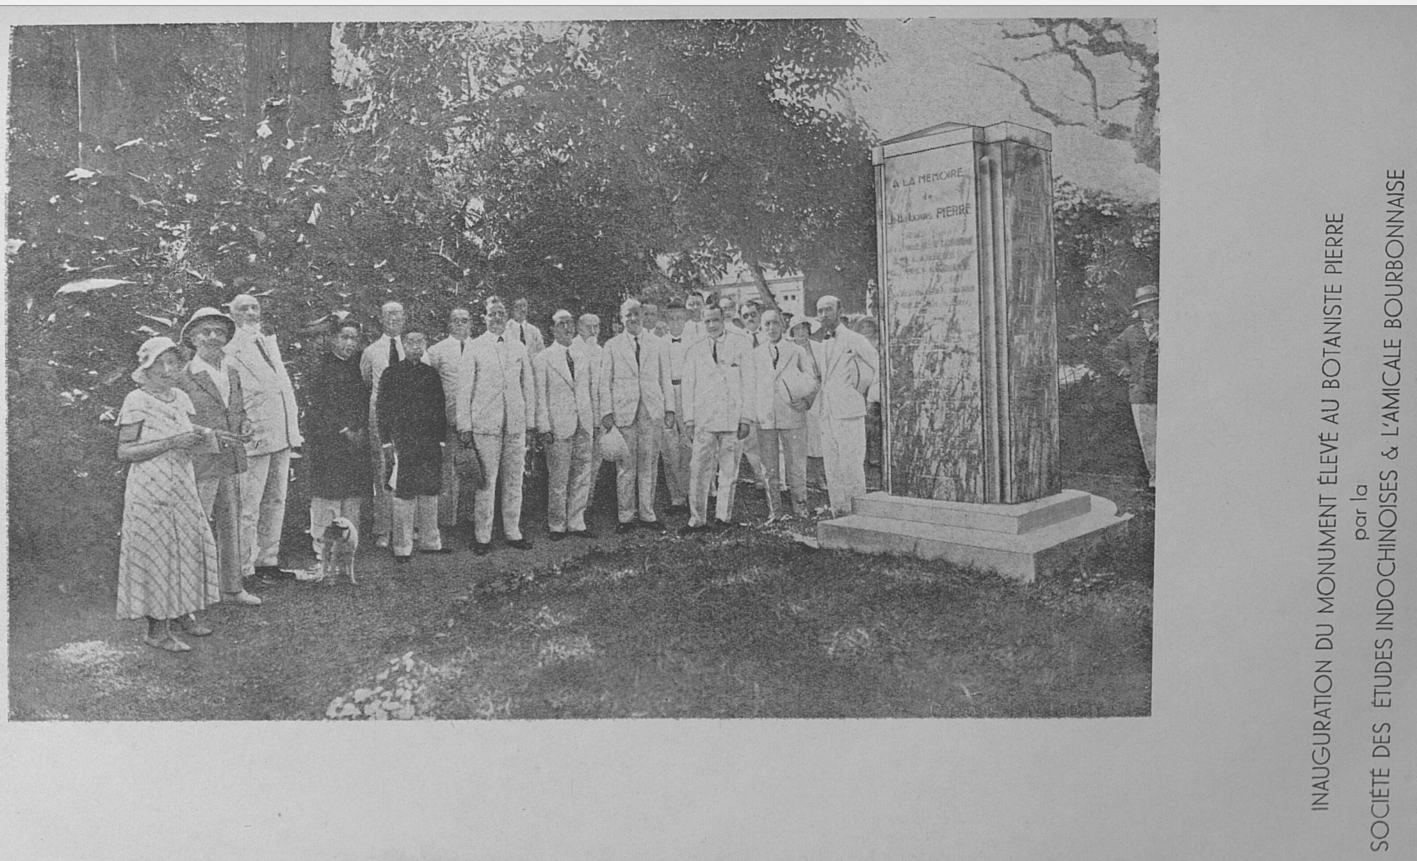
\includegraphics[width=1\linewidth]{img/société des études indochinoise.PNG}
    \caption{Société des études indochinoises et l'amical Bourbonnaise}
    \label{fig:enter-label}
\end{figure}

\begin{figure}[H] %[!ht]
    \centering
    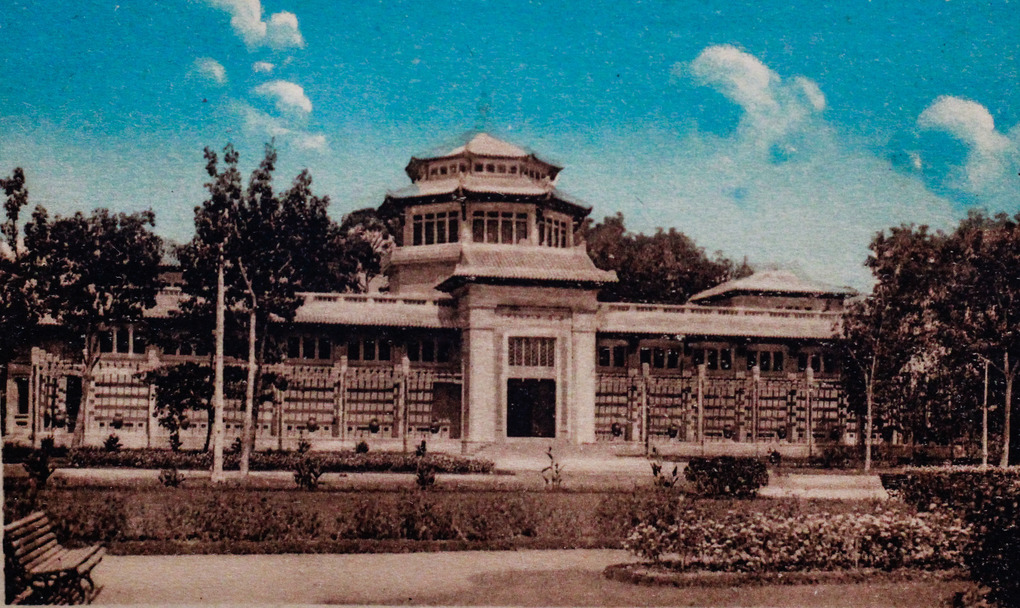
\includegraphics[width=1\linewidth]{img/museee.jpg}
    \caption{Musée Blanchard de la brosse}
    \label{fig:enter-label}
\end{figure}
souce : https://virtual-saigon.net/Data/Buildings?ID=4027

\begin{figure}[H] %[!ht]
    \centering
    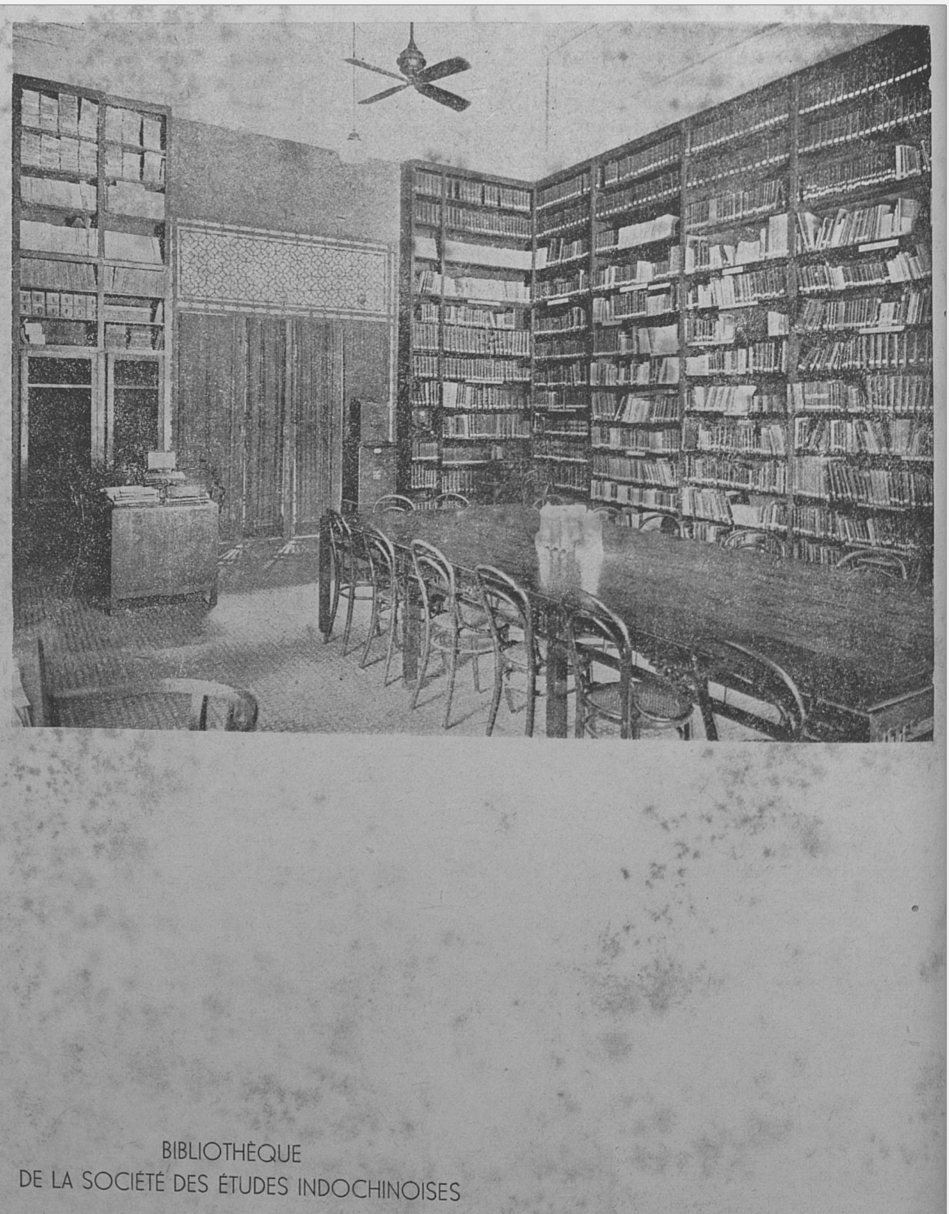
\includegraphics[width=1\linewidth]{img/bibliotheque.PNG}
    \caption{La bibliothèque de la société des études indochinoises}
    \label{fig:enter-label}
\end{figure}

\newpage
\section{Certains auteurs importants de B.S.E.I}

(La plupart des informations sur les autres sont collectées depuis Wikipedia)

\textbf{Maurice Durand} professeur de lettres au lycée Chasseloup-Lauba. Il est ensuite appelé auprès du recteur de l'université indochinoise, commet chef du bureau des affaires culturelles (1946-1947). Il est mémoire permanente de l’EFEO en 1949. Son œuvre scientifique est considérable. Il publie des études de grammaire, d'histoire, d'histoire des religions et d'histoire de l'art, ainsi que de traduction d'un roman classique en vers.
%%https://www.efeo.fr/biographies/notices/durand.htm

\textbf{Henri Marchal} (1876-1970)est un architecte français, mais aussi un explorateur, un archéologue et un philologue et épigraphe affecté à la Conservation d'Angkor, site sur lequel il travailla pendant plus de 40 ans jusqu'à un âge très avancé et donc, membre de l'École française d'Extrême-Orient. Il est décédé à Siem Reap (Cambodge) en 1970.

\textbf{Arthur Achéon} : administrateur de la 1e classe de Services civile de l'Indochine, un connaisseur remarquable de la langue annamite et un correspondant de l'Ecole Française d'Extrême-Orient.
%%https://www.persee.fr/doc/befeo_0336-1519_1928_num_28_3_3161

\textbf{Truong Vinh Tong} (1884-1974) était un professeur et homme politique vietnamien. Il a été ministre des Affaires étrangères du Vietnam sous la présidence de Nguyen Van Tam. Il était le plus jeune fils du savant vietnamien Pétrus Ky.

\textbf{Vuong Hong Sen} (1902-1996) avait trois lignées : Kinh, Chinois et Khmer. Durant ses années d'étudiant, il étudia au Collège Chasseloup Laubat. Après avoir obtenu le Brevet Elémentaire, il travaille comme fonctionnaire avec rang de secrétaire et sert dans de nombreux lieux de 1923 à 1943, notamment au Palais du Gouverneur de Cochinchine (1939 - 1943). À partir de 1948, il a travaillé comme conservateur par intérim du Musée national du Vietnam à Saigon jusqu'à sa retraite en 1964. Il était un lecteur assidu et aimait enregistrer tout ce qu'il entendait et voyait. La plupart de ses œuvres sont tirées de documents sous forme de mémoires qu'il conserve encore.

\textbf{Pétrus Truong Vinh Ky} (1837 - 1898) était un homme politique, érudit, écrivain, linguiste, éducateur et chercheur culturel vietnamien du XIXe siècle.
Tran Van Khe (1921-2015) était un célèbre chercheur en musique et culture traditionnelles au Vietnam. Il est le premier Vietnamien à avoir un doctorat en musicologie en France et a été professeur à l'Université de la Sorbonne, en France, et membre honoraire du Conseil international de la musique de l'UNESCO. C'est une personne avec une longue histoire d'activités de recherche et d'enseignement et a contribué à promouvoir la musique vietnamienne en particulier et la culture vietnamienne en général dans le monde.

\textbf{Nghiem Toan} (1907 - 1975) était un enseignant, professeur et chercheur littéraire qui a enseigné au lycée Gia Long, au lycée Van Lang, à l'Université de littérature de Saigon et à l'Université pédagogique de Saigon. Il porte également le pseudonyme de Hao Nhien.

\textbf{Nguyen The Anh} (1936-2023) est un écrivain vietnamien. Ancien recteur de l'université de Hué, et ancien responsable de la chaire Histoires et civilisations de la péninsule indochinoise à l'École pratique des hautes études à Paris, il est l'auteur de nombreuses études historiques en anglais, français et vietnamien.

\textbf{Thai Van Kiem} (1922-2015) est un orientaliste vietnamien originaire de Hue, ancien administrateur en chef des services civils du Vietnam et auteur de nombreux ouvrages sur la culture et la civilisation vietnamiennes.
\newpage 
\section{Certains présidents de la société}

\textbf{Doan-Quan-Tân (1895 - 1970)} était un éducateur, homme politique et fonctionnaire vietnamien. Ministre de l'Éducation nationale du gouvernement provisoire du Sud-Vietnam de 1948 à 1949, Directeur général de l'Agence d'information Vietnam-Presse de 1952 à 1954, et Conservateur de la Bibliothèque nationale du Sud-Vietnam de 1954 à 1957. Il a également été nommé Professeur au Lycée Jean-Jacques Rousseau de Saïgon en 1957.
Il était un membre actif de nombreuses organisations, y compris l'École française d'Extrême-Orient, la Société d'enseignement mutuel du Sud-Vietnam, l'Université populaire franco-vietnamienne, la Société des études indochinoises et l'Alliance Française. En reconnaissance de ses contributions, il a été fait Chevalier de la Légion d'honneur en 1955 et a reçu la médaille d'Officier d'académie la même année.
Enfin, le 5 décembre 1958, il est devenu membre non résidant de l'Académie des sciences d'outre-mer.

\textbf{PÂRIS Pierre Paul ( 1860-1943)}
Député de la Cochinchine de 1910 à 1914.
Commis-rédacteur aux affaires indigènes de Cochinchine en 1882, il fut adjoint en 1884 au représentant du Protectorat français au Cambodge. Administrateur en 1884, il exerça la fonction de résident général par intérim en 1886, mais il démissionna en 1887 pour se faire inscrire avocat au barreau de Saïgon.
Simultanément, il dirigea une plantation de caoutchouc et s'intéressa à la culture du riz.

\textbf{Raphaël Barquissau (1888 - 1961)} était un professeur français originaire de Saint-Pierre, La Réunion. Il était le fils de Lucien Barquissau, professeur à Saint-Pierre, et d'Adèle Barre.
Raphaël Barquissau a également occupé la présidence et la vice-présidence de plusieurs associations, dont l'Académie de la paix, la Société des agrégés de France, la Confédération des travailleurs intellectuels, l'Association nationale des écrivains d'expression française de la mer et de l'outre-mer, ainsi que la Société des poètes français. Il a également été délégué de la Société des études indochinoises.
Il est devenu membre titulaire de l'Académie des sciences coloniales le 4 mai 1945. En reconnaissance de ses contributions, il a été nommé chevalier de la Légion d'honneur en 1934, puis élevé au grade d'officier en 1949.

\textbf{Georges Paul Emile Lucien Gayet (1891 - 1962)} était un inspecteur de 1ère classe des colonies françaises. Né à Toulon, dans le Var, il était le fils de Pierre Emile Lucien Gayet et de Marie Christine Jeanne Valague, tous deux sans profession.
Il a notamment été chef du cabinet du Président du conseil et des ministres de la Marine et de l'Intérieur en 1933-1934, ainsi que directeur au ministère de l'Intérieur l'année suivante, avec des missions dans le sud algérien.
De 1947 à 1949, il a exercé les fonctions de chef de la mission de contrôle de l'exécution du budget de l'État en Indochine, participant à la conférence de Fontainebleau à la fin de la guerre d'Indochine. En 1950-1951, il a été commissaire du gouvernement près le conseil d'État pour le ministère de la France d'outre-mer.
En parallèle de sa carrière, Georges Paul Emile Lucien Gayet a également été actif dans plusieurs organisations, présidant la Société d'études indochinoises entre 1946 et 1949, ainsi que l'Académie de la Paix et le conseil consultatif du Comité central français pour l'outre-mer.
Il est devenu membre titulaire de la 2e section de l'Académie des sciences d'outre-mer le 19 juillet 1946.


\newpage 
\section{Project Vietnamica}\label{chapitre}

\bigskip

Je remercie toute l'équipe de Vietnamica et en particulier Philippe Papin, Marc Bui et Pascal Bourdeaux pour m'avoir permis de réaliser mes recherches sur leur corpus. 

\bigskip

\textbf{Équipe de Vietnamica en France:}
\begin{itemize}
    \item Philippe Papin
    \item Marc Bui
    \item Pascal Bourdeaux
    \item Nguyen Thi Hiep
    \item Béatrice Wisniewski
    \item Nguyen Thi Hai
    \item Lou Vargas
    \item Nguyen Hoang Phuc
    \item Jade Thau
    \item Olivier Masson
    \item Ho Kim Thoa
\end{itemize}

\bigskip

Lien : \url{https://vietnamica.online/}.

\bigskip

\newpage 
\section{Regroupement des disciplines scientifiques}
Dans le tableau \ref{tab:full_discipline}, nous répertorions les résultats de la recherche de documents portant sur diverses disciplines scientifiques obtenus grâce à la combinaison de deux modèles, Top2Vec et Word2Vec. Nous ne présentons ici que les articles dont le score de similarité dépasse 0,3, une valeur que nous avons établie après observation et estimation, et qui permet d'obtenir une indication satisfaisante de la pertinence du document par rapport au sujet auquel il a été classifié.

\begin{longtable}{|p{3cm}|p{1cm}|p{10cm}|p{1cm}|}
\hline
Discipline & Score & Articles & Année\\
\hline
anatomie & 0.61 & l extrême asie et le corps humain 1948 tome xxiii & 1948  \\ \hline
anatomie & 0.47 & quelques aspects de la pénétration des sciences occidentales au japon depuis le xvie siècle 1952 tome xxvii & 1952  \\ \hline
anatomie & 0.36 & lãn ông et la médecine sino vietnamienne 1953 tome xxviii & 1953  \\ \hline
anatomie & 0.32 & etudes anthropologiques 1951 tome xxvi & 1951  \\ \hline
anatomie & 0.32 & bibliographie etudes historiques sur l ancienne médecine au viêt nam et en chine 1955 tome xxx & 1955  \\ \hline
anatomie & 0.31 & bio bibliographie de la médecine chinoise 1956 tome xxxi & 1956  \\ \hline
anatomie & 0.31 & extrait d une lettre de m josselme en réponse aux observations de m viaud 1888 semestre 2 & 1888  \\ \hline
anatomie & 0.30 & les chemins du raisonnement et de la logique en extrême orient 1949 tome xxiv & 1949  \\ \hline
anthropologie & 0.41 & anthropologie physique des chams 1951 tome xxvi & 1951  \\ \hline
anthropologie & 0.40 & raciologie de l indochine française 1947 tome xxii & 1947  \\ \hline
anthropologie & 0.39 & etudes anthropologiques 1951 tome xxvi & 1951  \\ \hline
anthropologie & 0.34 & variétés internationales 1960 tome xxxv & 1960  \\ \hline
anthropologie & 0.32 & variétés 1959 tome xxxiv 4 & 1959  \\ \hline
anthropologie & 0.31 & ixe congrès des sciences du pacifique bui quang tung 1957 tome xxxii & 1957  \\ \hline
archéologie & 0.43 & etudes archéologiques indiennes 1951 tome xxvi & 1951  \\ \hline
archéologie & 0.39 & sociétés savantes en rapport avec la société des etudes indochinoises de saigon 1884 semestre 1 & 1884  \\ \hline
archéologie & 0.36 & etudes indochinoises 1951 tome xxvi & 1951  \\ \hline
archéologie & 0.35 & bibliographie 1928 tome iii & 1928  \\ \hline
archéologie & 0.34 & catalogue des collections reliées 1887 semestre 2 & 1887  \\ \hline
archéologie & 0.34 & la vie et l œuvre de louis malleret 1901 1970 1971 tome xlvi & 1971  \\ \hline
archéologie & 0.34 & variétés 24e congrès international des orientalistes munich 1957 1957 tome xxxii & 1957  \\ \hline
archéologie & 0.34 & la vie et l œuvre de henri parmentier 1871 1949 1949 tome xxiv & 1949  \\ \hline
archéologie & 0.34 & adresses de félicitations des sociétés savantes d indochine et d outre mer 1933 tome viii & 1933  \\ \hline
archéologie & 0.34 & echanges 1933 tome viii & 1933  \\ \hline
archéologie & 0.33 & le musée ethnographique de la sei 1932 tome vii & 1932  \\ \hline
archéologie & 0.33 & congrès international d histoire des relations culturelles entre l occident et l orient s de labrusse 1957 tome xxxii & 1957  \\ \hline
archéologie & 0.32 & catalogue des collections reliées 1887 semestre 1 & 1887  \\ \hline
archéologie & 0.31 & la vie et l œuvre de george coedès 1886 1969 1971 tome xlvi & 1971  \\ \hline
archéologie & 0.30 & variétés bibliographiques 1940 tome xv & 1940  \\ \hline
astrobiologie & 0.62 & variété bibliographiques 1936 tome xi 4 & 1936  \\ \hline
astrobiologie & 0.31 & bio bibliographie de la médecine chinoise 1956 tome xxxi & 1956  \\ \hline
astronomie & 0.40 & variété bibliographiques 1936 tome xi 4 & 1936  \\ \hline
astronomie & 0.40 & la pensée scientifique en asie ancienne 1953 tome xxviii & 1953  \\ \hline
astronomie & 0.37 & vérification des dates des inscriptions des monuments khmers seconde partie 1910 semestre 1 & 1910  \\ \hline
astronomie & 0.33 & quelques aspects de la pénétration des sciences occidentales au japon depuis le xvie siècle 1952 tome xxvii & 1952  \\ \hline
astronomie & 0.32 & etude sur la vérification des dates des inscriptions des monuments khmers 1909 semestre 2 & 1909  \\ \hline
économiste & 0.45 & catalogue des collections reliées 1887 semestre 2 & 1887  \\ \hline
économiste & 0.42 & catalogue des collections reliées 1887 semestre 1 & 1887  \\ \hline
économiste & 0.38 & une enquête démographique et sociale sur un quartier de saigon cholon 1954 tome xxix & 1954  \\ \hline
économiste & 0.36 & variétés au viêt nam variétés internationales 1961 tome xxxvi & 1961  \\ \hline
ethnographie & 0.41 & echanges 1933 tome viii & 1933  \\ \hline
ethnographie & 0.36 & l exposition ethnographique de la société des etudes indochinoises 1933 tome viii & 1933  \\ \hline
ethnographie & 0.33 & note sur le missionnaire charles emile bouillevaux découvreur d angkor 1949 tome xxiv & 1949  \\ \hline
ethnographie & 0.32 & raciologie de l indochine française 1947 tome xxii & 1947  \\ \hline
ethnographie & 0.32 & le musée ethnographique de la sei 1932 tome vii & 1932  \\ \hline
ethnographie & 0.32 & rapport financier pour l année 1933 1934 tome ix 3 & 1934  \\ \hline
ethnologie & 0.43 & introduction à l ethnologie du đình 1962 tome xxxvii & 1962  \\ \hline
ethnologie & 0.41 & notes bibliographiques 1951 tome xxvi & 1951  \\ \hline
ethnologie & 0.38 & congrès international d histoire des relations culturelles entre l occident et l orient s de labrusse 1957 tome xxxii & 1957  \\ \hline
ethnologie & 0.33 & l orientalisme et les sciences humaines 1951 tome xxvi & 1951  \\ \hline
ethnologie & 0.33 & variétés 1959 tome xxxiv 4 & 1959  \\ \hline
ethnologie & 0.31 & adresses de félicitations des sociétés savantes d indochine et d outre mer 1933 tome viii & 1933  \\ \hline
ethnologie & 0.31 & variétés internationales 1960 tome xxxv & 1960  \\ \hline
géographie & 0.61 & sociétés savantes en rapport avec la société des etudes indochinoises de saigon 1884 semestre 1 & 1884  \\ \hline
géographie & 0.58 & catalogue des collections reliées 1887 semestre 1 & 1887  \\ \hline
géographie & 0.56 & catalogue des collections reliées 1887 semestre 2 & 1887  \\ \hline
géographie & 0.52 & echanges 1933 tome viii & 1933  \\ \hline
géographie & 0.35 & séance de commémoration du cinquantenaire de la société des etudes indochinoises 1883 1933 1933 tome viii & 1933  \\ \hline
géographie & 0.35 & etudes géographiques 1951 tome xxvi & 1951  \\ \hline
géographie & 0.32 & variétés 1958 tome xxxiii & 1958  \\ \hline
géographie & 0.32 & hanoi notes de géographie urbaine 1955 tome xxx & 1955  \\ \hline
géographie & 0.31 & bibliographie de l indo chine orientale depuis 1880 1889 semestre 1 & 1889  \\ \hline
linguistique & 0.45 & structure de la langue vietnamienne 1974 tome xlix & 1974  \\ \hline
linguistique & 0.44 & l orientalisme et les sciences humaines 1951 tome xxvi & 1951  \\ \hline
linguistique & 0.34 & articles récents sur l asie du sud est 8 1973 tome xlviii & 1973  \\ \hline
linguistique & 0.32 & une étape importante en linguistique vietnamienne 1972 tome xlvii & 1972  \\ \hline
linguistique & 0.32 & etudes centre asiatiques 1951 tome xxvi & 1951  \\ \hline
linguistique & 0.32 & carte ethno linguistique de la région de voeunsai cambodge 1952 tome xxvii & 1952  \\ \hline
linguistique & 0.31 & les formes de politesse en javanais moderne 1950 tome xxv & 1950  \\ \hline
linguistique & 0.30 & bibliographie 1965 tome xl & 1965  \\ \hline
mathématique & 0.45 & quelques aspects de la pénétration des sciences occidentales au japon depuis le xvie siècle 1952 tome xxvii & 1952  \\ \hline
mathématique & 0.37 & la science au viêt nam 1963 tome xxxviii & 1963  \\ \hline
mathématique & 0.37 & l extrême asie et le corps humain 1948 tome xxiii & 1948  \\ \hline
mathématique & 0.31 & variété bibliographiques 1936 tome xi 4 & 1936  \\ \hline
mathématique & 0.31 & alexandre de rhodes 1957 tome xxxii & 1957  \\ \hline
médecine & 0.58 & lãn ông et la médecine sino vietnamienne 1953 tome xxviii & 1953  \\ \hline
médecine & 0.50 & bio bibliographie de la médecine chinoise 1956 tome xxxi & 1956  \\ \hline
médecine & 0.41 & de la diffusion de la médecine européenne en cochinchine 1895 3e fascicule & 1895  \\ \hline
médecine & 0.41 & histoire de l acupuncture chinoise 1959 tome xxxiv & 1959  \\ \hline
médecine & 0.41 & bibliographie etudes historiques sur l ancienne médecine au viêt nam et en chine 1955 tome xxx & 1955  \\ \hline
médecine & 0.33 & quelques aspects de la pénétration des sciences occidentales au japon depuis le xvie siècle 1952 tome xxvii & 1952  \\ \hline
médecine & 0.32 & panorama médical du viêt nam d autrefois 1951 tome xxvi & 1951  \\ \hline
médecine & 0.32 & médecine populaire au cambodge 1965 tome xl & 1965  \\ \hline
nationaliste & 0.40 & congrès international d histoire des relations culturelles entre l occident et l orient s de labrusse 1957 tome xxxii & 1957  \\ \hline
nationaliste & 0.38 & la science au viêt nam 1963 tome xxxviii & 1963  \\ \hline
nationaliste & 0.34 & bibliographie dictionnaires vietnamiens 1972 tome xlvii & 1972  \\ \hline
nationaliste & 0.31 & les formes de politesse en javanais moderne 1950 tome xxv & 1950  \\ \hline
orientaliste & 0.36 & variétés 24e congrès international des orientalistes munich 1957 1957 tome xxxii & 1957  \\ \hline
orientaliste & 0.32 & l orientalisme et les sciences humaines 1951 tome xxvi & 1951  \\ \hline
paléontologie & 0.61 & le révérend père emile licent sj 1966 tome xli & 1966  \\ \hline
paléontologie & 0.46 & le service géologique de l indochine 1898 1953 le service géologique de la république du viêt nam depuis 1953 1973 tome xlviii & 1973  \\ \hline
paléontologie & 0.39 & bibliographie 1960 tome xxxv & 1960  \\ \hline
paléontologie & 0.32 & le paléolithique des environs de xuân loc 1971 tome xlvi & 1971  \\ \hline
philologie & 0.45 & in mémoriam jean przylusky 1946 tome xxi & 1946  \\ \hline
philologie & 0.38 & congrès international d histoire des relations culturelles entre l occident et l orient s de labrusse 1957 tome xxxii & 1957  \\ \hline
philologie & 0.38 & le musée ethnographique de la sei 1932 tome vii & 1932  \\ \hline
philologie & 0.33 & etudes indiennes classiques 1951 tome xxvi & 1951  \\ \hline
philologie & 0.32 & maurice durand 1914 1966 1966 tome xli & 1966  \\ \hline
philologie & 0.31 & rapports de l étude pratique de la langue annamite vulgaire 1884 semestre 1 & 1884  \\ \hline
philologue & 0.46 & etudes chinoises classiques 1951 tome xxvi & 1951  \\ \hline
philologue & 0.43 & paul pelliot 1946 tome xxi & 1946  \\ \hline
philologue & 0.42 & etudes indiennes classiques 1951 tome xxvi & 1951  \\ \hline
philologue & 0.32 & in memoriam alfred foucher 1952 tome xxvii & 1952  \\ \hline
philologue & 0.31 & l orientalisme et les sciences humaines 1951 tome xxvi & 1951  \\ \hline
philosophie & 0.41 & variété bibliographiques 1936 tome xi 4 & 1936  \\ \hline
philosophie & 0.35 & bibliographie dictionnaires vietnamiens 1972 tome xlvii & 1972  \\ \hline
philosophie & 0.31 & les chemins du raisonnement et de la logique en extrême orient 1949 tome xxiv & 1949  \\ \hline
précolombien & 0.52 & l amérique précolombienne et l asie méridionale 2e article 1943 tome xviii & 1943  \\ \hline
précolombien & 0.36 & rapport trimestriel 1942 tome xvii & 1942  \\ \hline
précolombien & 0.34 & table méthodique par matières 1949 tome xxiv & 1949  \\ \hline
précolombien & 0.32 & tables du bulletin de la sei 1971 tome xlvi & 1971  \\ \hline
préhistoire & 0.38 & présentation d ouvrages 1973 tome xlviii 4 & 1973  \\ \hline
préhistoire & 0.33 & chronique littéraire 1958 tome xxxiii & 1958  \\ \hline
préhistoire & 0.32 & raciologie de l indochine française 1947 tome xxii & 1947  \\ \hline
préhistoire & 0.31 & nouvelles récoltes d objets préhistoriques 1975 tome l & 1975  \\ \hline
sinologie & 0.70 & etudes chinoises classiques 1951 tome xxvi & 1951  \\ \hline
sinologie & 0.43 & paul pelliot 1946 tome xxi & 1946  \\ \hline
sinologie & 0.41 & etudes bouddhiques 1951 tome xxvi & 1951  \\ \hline
sinologie & 0.39 & nécrologie de maurice verdeille 1875 1940 1940 tome xv & 1940  \\ \hline
sinologie & 0.37 & bibliographie 1964 tome xxxix 2 & 1964  \\ \hline
sinologie & 0.32 & bibliographie 1960 tome xxxv & 1960  \\ \hline
sinologie & 0.31 & chronique littéraire 1959 tome xxxiv & 1959  \\ \hline
sociologie & 0.37 & bibliographie des livres et revues reçus en 1958 1959 tome xxxiv & 1959  \\ \hline
sociologie & 0.36 & revues 1962 tome xxxvii 1 & 1962  \\ \hline
sociologie & 0.33 & essai de bibliographie pratique sur les populations montagnardes du sud vietnam 1935 1966 1967 tome xlii & 1967  \\ \hline
sociologie & 0.32 & chronique littéraire 1958 tome xxxiii & 1958  \\ \hline
sociologie & 0.31 & articles récents sur l asie du sud est 8 1973 tome xlviii & 1973 \\ \hline 
\end{longtable}
\label{tab:full_discipline}